\subsection{System hardware details}
\label{sub:system-specs}
\begin{lstlisting}[language={}]
System:    Host: Hastings
           Kernel: 4.2.0-30-generic x86_64 (64 bit gcc: 5.2.1)
           Console: tty 2
           Distro: Ubuntu 15.10 wily
Machine:   System: Dell product: OptiPlex 960 serial: 1GCNK4J
           Mobo: Dell model: 0Y958C v: A00 serial: ..CN708219AMH0BL.
           Bios: Dell v: A05 date: 07/31/2009
CPU:       Dual core Intel Core2 Duo E8400 (-MCP-) cache: 6144 KB
           flags: (lm nx sse sse2 sse3 sse4_1 ssse3 vmx) bmips: 11969
           clock speeds: max: 3000 MHz 1: 2667 MHz 2: 2000 MHz
Memory:    Array-1 capacity: 8 GB devices: 4 EC: None
           Device-1: DIMM_1 size: 2 GB speed: 800 MHz type: DDR2 part: NT2GT64U8HD0BY-AD
           Device-2: DIMM_3 size: 2 GB speed: 800 MHz type: DDR2 part: NT2GT64U8HD0BY-AD
           Device-3: DIMM_2 size: 2 GB speed: 800 MHz type: DDR2 part: NT2GT64U8HD0BY-AD
           Device-4: DIMM_4 size: 2 GB speed: 800 MHz type: DDR2 part: NT2GT64U8HD0BY-AD
           Device-5: N/A size: N/A speed: N/A type: N/A part: N/A
Network:   Card: Intel 82567LM-3 Gigabit Network Connection
           driver: e1000e v: 3.2.5-k
           port: ecc0 bus-ID: 00:19.0
           IF: enp0s25 state: up
           speed: 1000 Mbps
           duplex: full mac: 00:26:b9:75:99:1b
Drives:    HDD Total Size: 320.1GB (6.2% used)
           ID-1: /dev/sda
           model: WDC_WD3200AAKS
           size: 320.1GB
           temp: 34C
           Optical: /dev/sr0
           model: PLDS DVD+-RW DH-16AAS
           rev: JD12
           dev-links: cdrom,cdrw,dvd,dvdrw

\end{lstlisting}

\subsection{Performance test of clientside JavaScript}
\begin{figure}[H]
    \centering
    \begin{subfigure}{0.49\textwidth}
        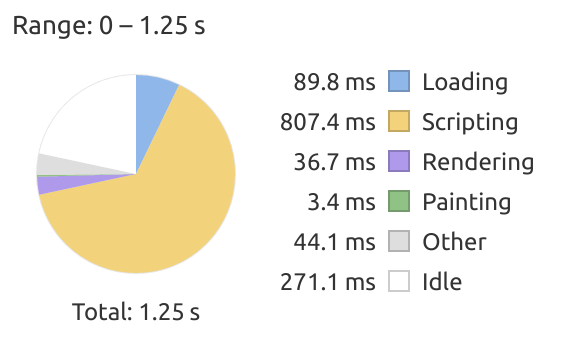
\includegraphics[width=\textwidth]{figure/clientsidePerformance/graph1.png}
    \end{subfigure}
    \begin{subfigure}{0.49\textwidth}
        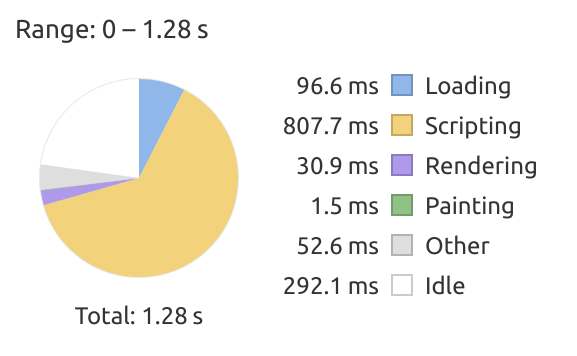
\includegraphics[width=\textwidth]{figure/clientsidePerformance/graph2.png}
    \end{subfigure}
    \\
    \begin{subfigure}{0.5\textwidth}
        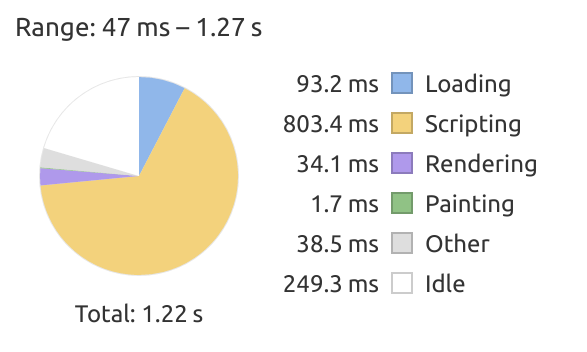
\includegraphics[width=\textwidth]{figure/clientsidePerformance/graph3.png}
    \end{subfigure}
    
    \caption{Loading hastings clientside javascript with no games and 1 player connected.}
    \label{fig:my_label}
\end{figure}

\begin{figure}[h!]
    \centering
    \begin{subfigure}{0.49\textwidth}
        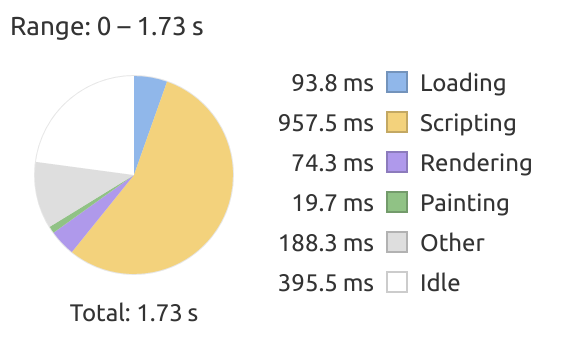
\includegraphics[width=\textwidth]{figure/clientsidePerformance/graph30games1.png}
    \end{subfigure}
    \begin{subfigure}{0.49\textwidth}
        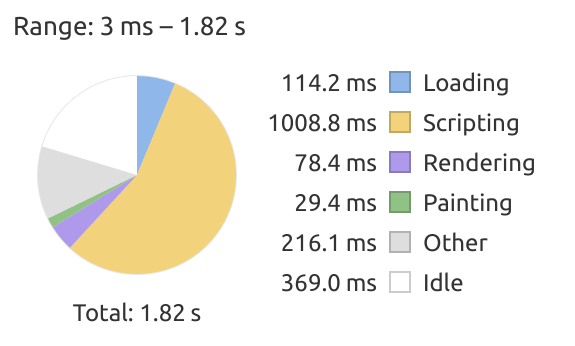
\includegraphics[width=\textwidth]{figure/clientsidePerformance/graph30games2.png}
    \end{subfigure}
    \\
    \begin{subfigure}{0.5\textwidth}
        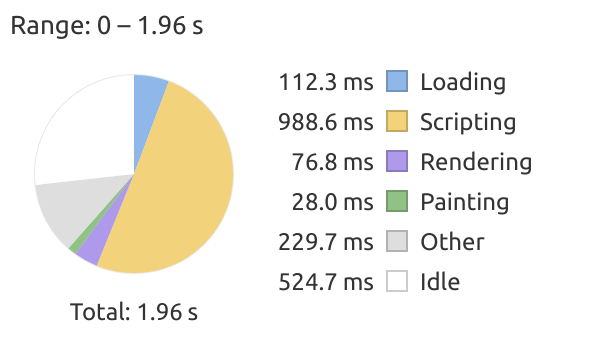
\includegraphics[width=\textwidth]{figure/clientsidePerformance/graph30games3.png}
    \end{subfigure}
    
    \caption{Loading hastings clientside javascript with 30 games and 1 player connected.}
    \label{fig:my_label}
\end{figure}

\begin{figure}[h!]
    \centering
    \begin{subfigure}{0.49\textwidth}
        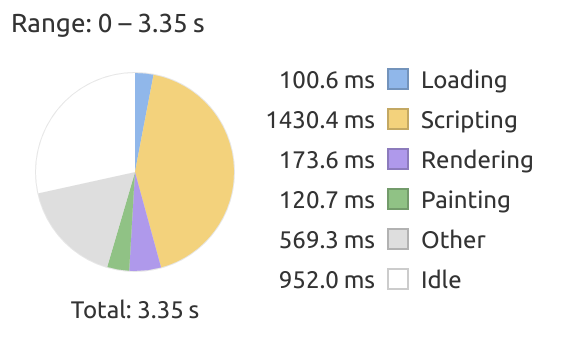
\includegraphics[width=\textwidth]{figure/clientsidePerformance/graph90games1.png}
    \end{subfigure}
    \begin{subfigure}{0.49\textwidth}
        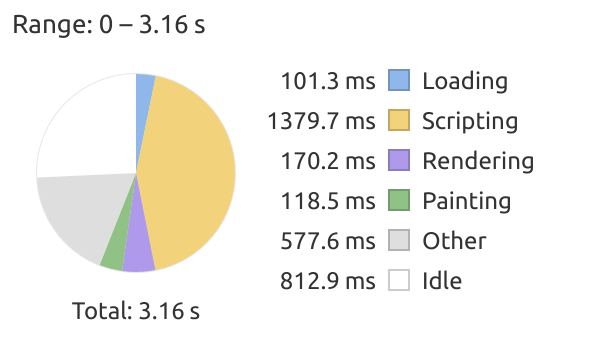
\includegraphics[width=\textwidth]{figure/clientsidePerformance/graph90games2.png}
    \end{subfigure}
    \\
    \begin{subfigure}{0.5\textwidth}
        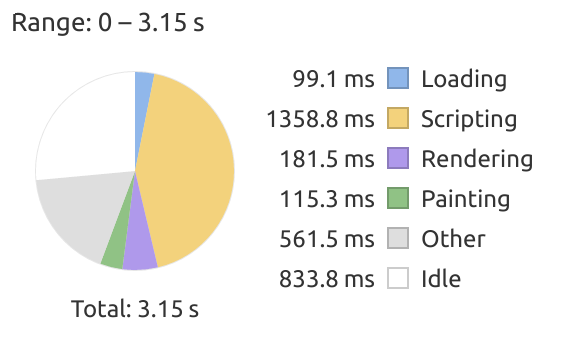
\includegraphics[width=\textwidth]{figure/clientsidePerformance/graph90games3.png}
    \end{subfigure}
    
    \caption{Loading hastings clientside javascript with 90 games and 1 player connected.}
    \label{fig:my_label}
\end{figure}

\begin{figure}[h!]
    \centering
    \begin{subfigure}{0.49\textwidth}
        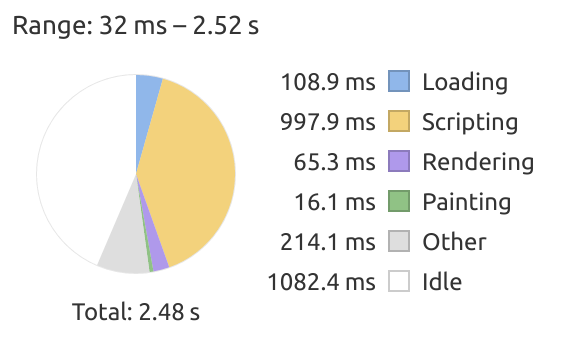
\includegraphics[width=\textwidth]{figure/clientsidePerformance/braseegraph1.png}
    \end{subfigure}
    \begin{subfigure}{0.49\textwidth}
        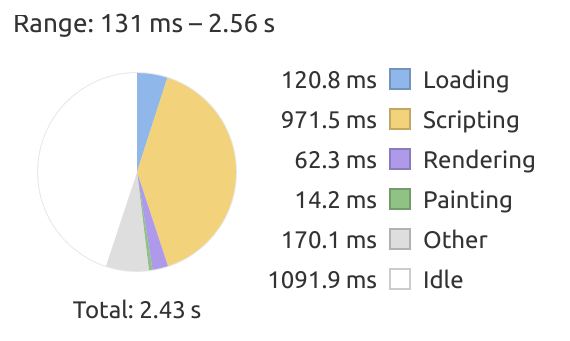
\includegraphics[width=\textwidth]{figure/clientsidePerformance/braseegraph2.png}
    \end{subfigure}
    \\
    \begin{subfigure}{0.5\textwidth}
        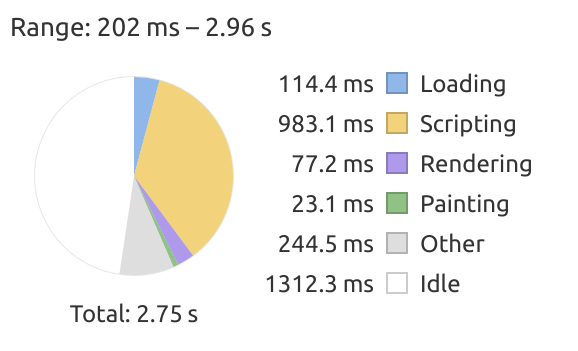
\includegraphics[width=\textwidth]{figure/clientsidePerformance/braseegraph3.png}
    \end{subfigure}
    
    \caption{Loading brasee.com lobby, with x players in it, not too many idk.}
    \label{fig:my_label}
\end{figure}

\begin{figure}[h!]
    \centering
    \begin{subfigure}{0.49\textwidth}
        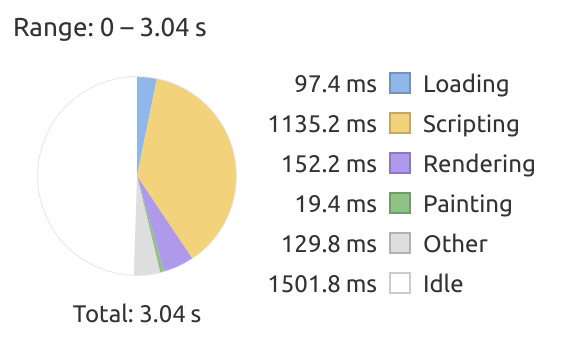
\includegraphics[width=\textwidth]{figure/clientsidePerformance/ligraph1.png}
    \end{subfigure}
    \begin{subfigure}{0.49\textwidth}
        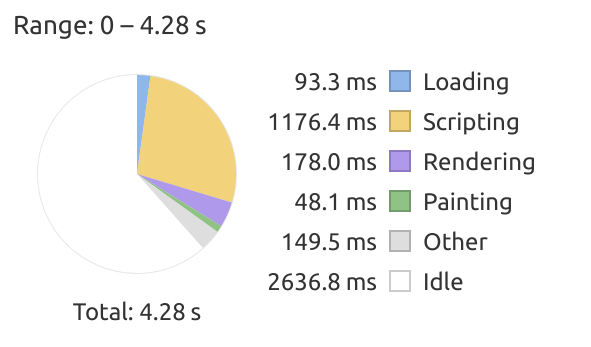
\includegraphics[width=\textwidth]{figure/clientsidePerformance/ligraph2.png}
    \end{subfigure}
    \\
    \begin{subfigure}{0.5\textwidth}
        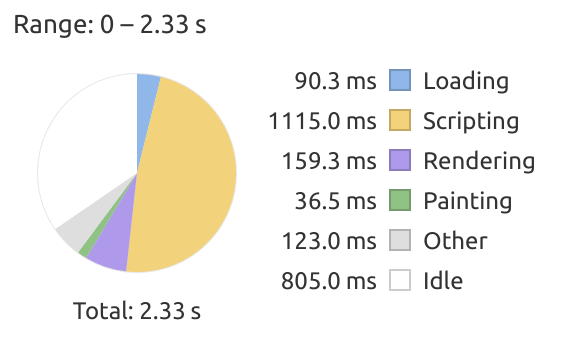
\includegraphics[width=\textwidth]{figure/clientsidePerformance/ligraph3.png}
    \end{subfigure}
    
    \caption{Loading lichess.org with approximately 6000 players and 1500 games, not all on frontpage though.}
    \label{fig:my_label}
\end{figure}

\subsection{Performance test of server side performance}
\begin{figure}
    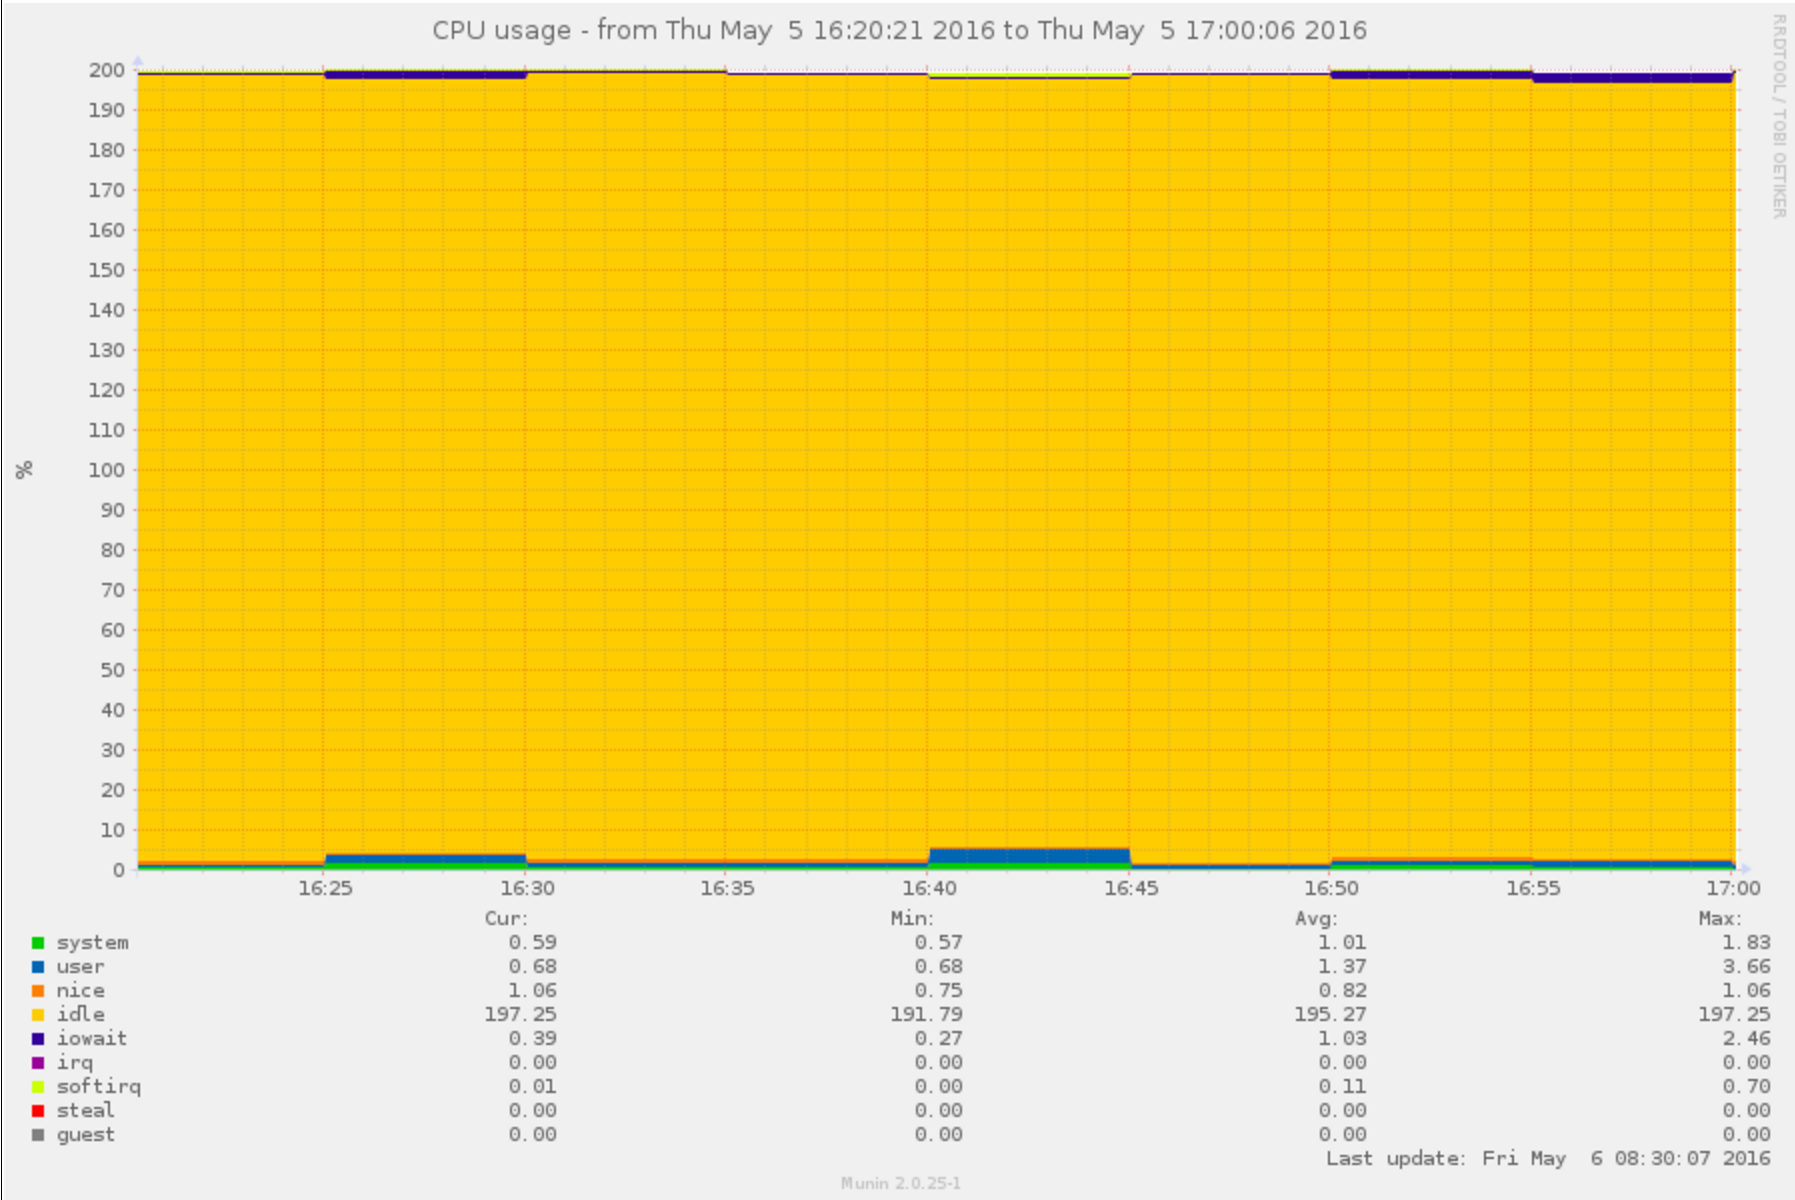
\includegraphics[width=\textwidth]{figure/serversidePerformance/2016-05-05-chatting-test-cpu.png}
    \caption{CPU usage during the chat test}
    \label{fig:cpu-results-attachment}
\end{figure}

\begin{figure}
    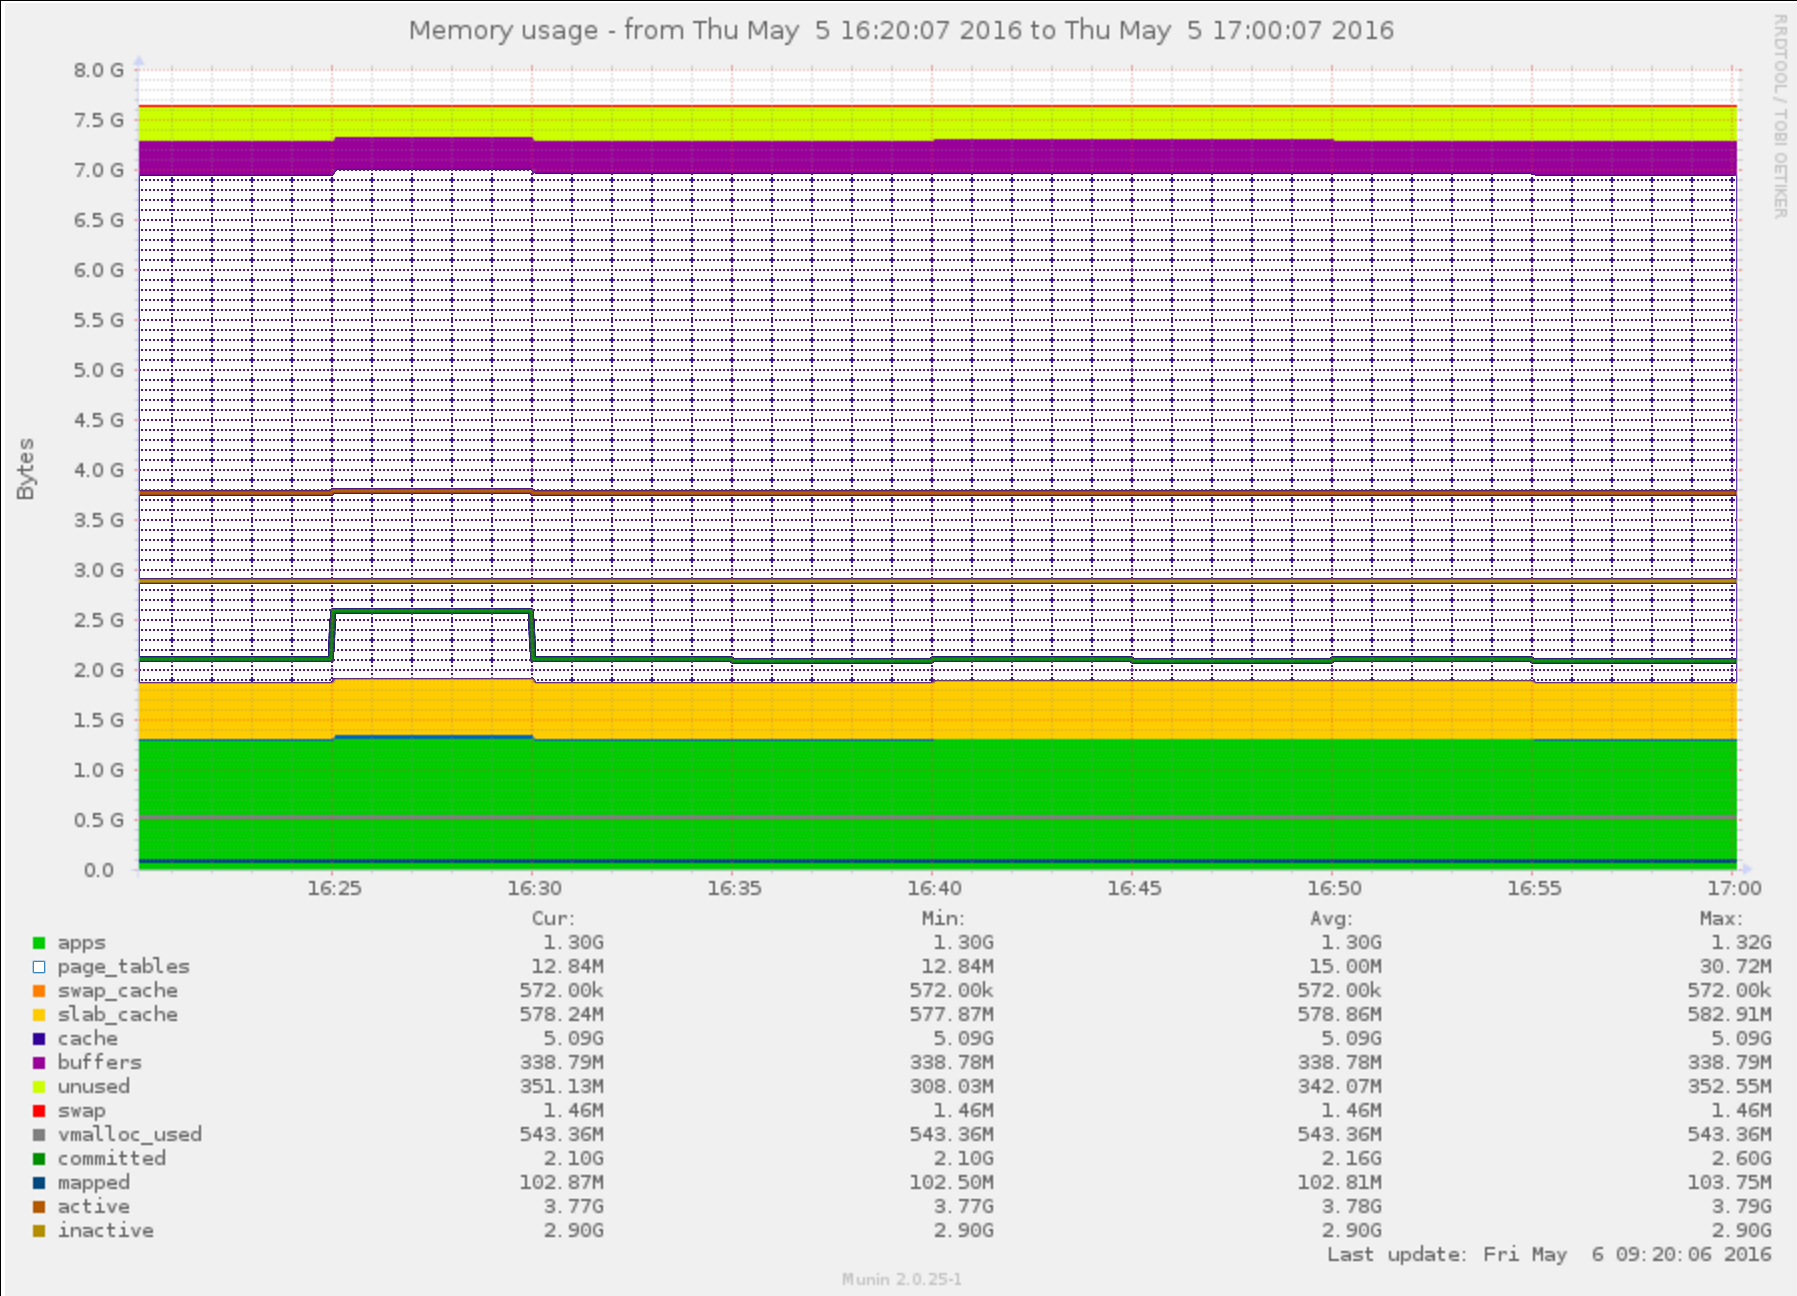
\includegraphics[width=\textwidth]{figure/serversidePerformance/2016-05-05-chat-memory.png}
    \caption{Memory usage on the server during the chat test}
    \label{fig:memory-results-attachment}
\end{figure}


\begin{figure}
    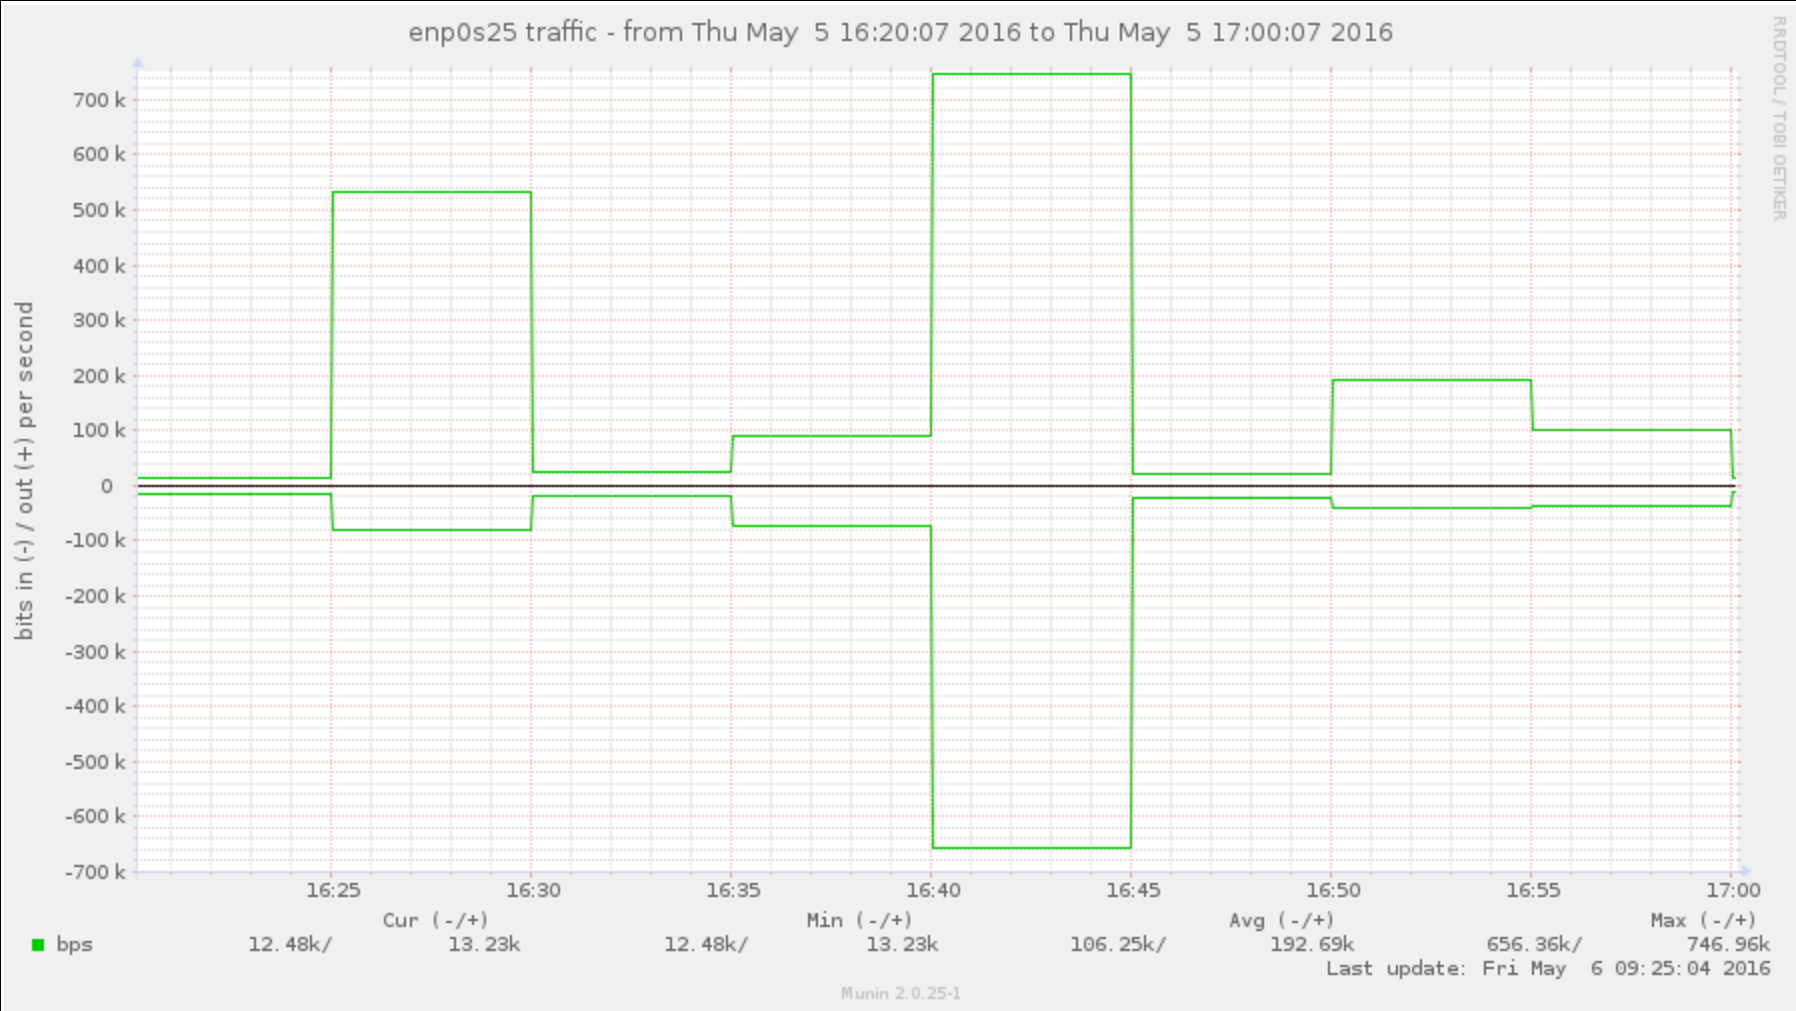
\includegraphics[width=\textwidth]{figure/serversidePerformance/2016-05-05-network-traffic-chat.png}
    \caption{Network traffic on the server during the chat test}
    \label{fig:network-results-attachment}
\end{figure}

\begin{figure}
    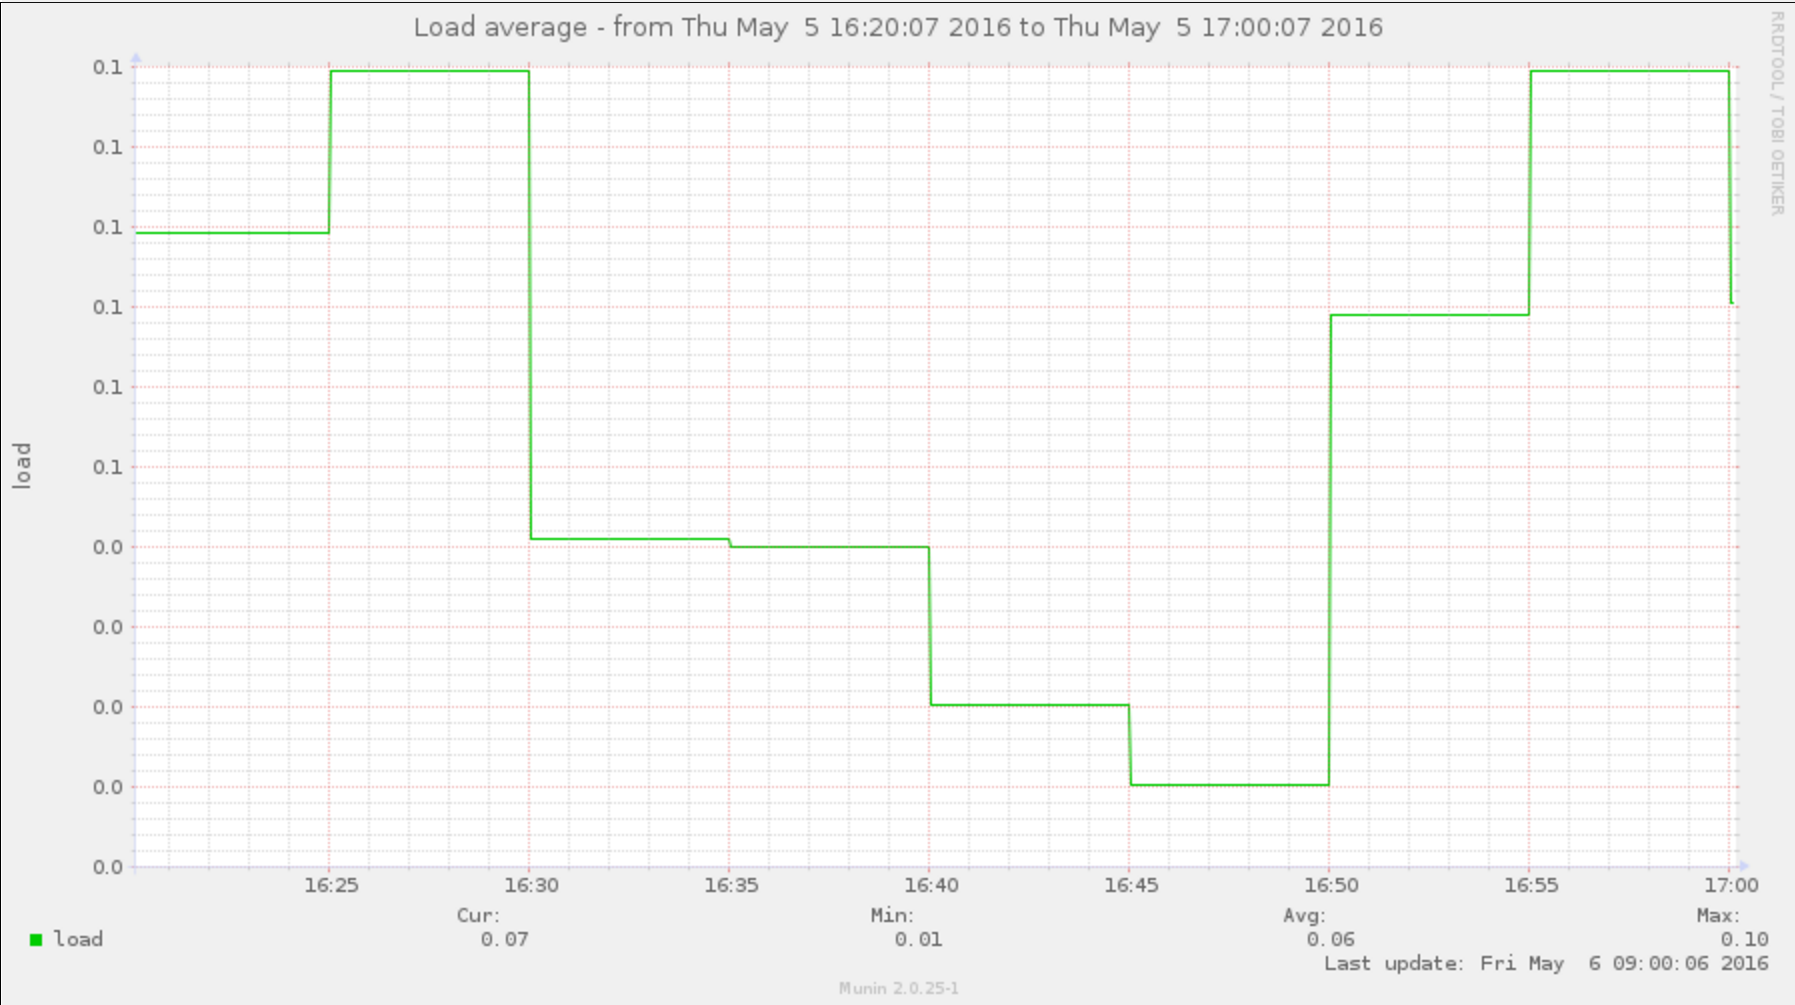
\includegraphics[width=\textwidth]{figure/serversidePerformance/2016-05-05-load-average-chatting-tests.png}
    \caption{Load average on the server during the chat test}
    \label{fig:load-average-results-attachment}
\end{figure}

\section{Mattias Nilsen, bidragsrapport}
\subsection{Ansvarsområden}
Jag hade rollen som projektledare vilket framförallt har inneburit att vara ordförande på möten samt hålla kontakt med handledare och andra personer utanför gruppen.
Vid implementering av applikationen har jag bara arbetat med lobbydelen, jag har varit skrivit kod i nästan alla delar av lobbyn. Jag är dock ensam ansvarig för databasimplementationen för lobbyn.
Utöver att koda har jag även utfört kodrecension på den kod som andra skrivit till lobbyn innan den har fått appliceras på applikationen.

Jag har varit med i alla stadier från idé till färdig applikation och rapport.
Skapande av en modell, analys av resultat och bidrag med nya ideer har jag bidragit med i lika stor utsträckning som de andra i gruppen.
Jag är delansvarig för den muntliga slutredovisningen.

Nedan följer en lista med delar jag har skrivit nästan helt på egen hand följt av de avsnitt där jag bidragit med text men inte skrivit allt själv.
Jag har utöver detta gjort redaktionella ändringar i nästan alla avsnitt i rapporten.

\begin{itemize}
    \item Gjort layouten på framsidan i Latex
    \item 3.2 JavaScript
    \item 3.6 SQL & MySQL
    \item 6.2.3 Client-side performance
    \item 6.4.2 Runtime errors and debugging
    \item 6.4.3 Database usage influence on programmer productivity
    \item 7.1.5 Measuring programmer productivity
\end{itemize}

\begin{itemize}
    \item 1.1 Background
    \item 4.1 How To Measure Performance
    \item 5.1 Dependency Management Using Haste.App
    \item 5.4 Development of the lobby system - Skrev delen om databashantering
    \item 6.1 Game and Lobby implementation results
    \item 6.4.4 A client-centric, seamless, and linear program flow
    \item 7.1.3 Measuring performance
    \item 7.2.1 Performance of Haste.App
    \item 7.2.3 Programmer productivity when working with Haste.App
\end{itemize}


